
\documentclass[11pt]{article}
\usepackage{float}
\usepackage{graphicx}
%Gummi|061|=)
\title{\textbf{Homework 3}}
\author{Max Espinoza}
\date{}
\begin{document}

\maketitle

\section{Background}

\hspace{4ex}The visual data set I choose was based on a paper published by Cem Yuksel published in SIGGRAPH on \textbf{Wave Particles}.
Yuksel used these "wave particles" to implement a real time water simulation with buoyant forces. 
Yuksel simulation took advantage of the ease of computation of particles over solving the wave equation for water simulations.
He creates his mesh for water simulations by creating an extended height field. This height field can be mathematically solved for accuracy, however Yuksel looking for an interactive way to simulate water, uses water particles to solve for the local deviation functions.
To simplify how Yuksel creates his water simulation we must first look at the how he defines his extended height field.

% Insert equation 2
\begin{equation}
z(\textbf{x},t) = z_0 + n_z(\textbf{x},t)
\end{equation}

This height field is sum of base height $z_0$ with the deviation function $n_z$ given a specific coordinate and time.
The deviation field is defined as follows.

\begin{equation}
n_z(\textbf{x},t) = \sum\limits_{i} D_i(\textbf{x},t)
\end{equation}

In order to find the deviation field ( the sum of the local deviation functions ) we must either analytically solve for each local deviation function or rely on wave particles to approximate this for us.
The local deviation function is defined below. I see this mathematically how much a wave particle has influence over the result of the hight field. Note there is also a blending function I didn't implement because I'm not looking to create wave surfaces but instead apply wave particles to audio visualizations.
\begin{equation}
D_i(x,t) = a_i W_i(x-x_i(t))
\end{equation}


The novelty in Yuksel work is the relation of wave particles with this local deviation functions.
Being able to use wave particles over solving for the wave equation allows save us a lot of computational time. Despite the lost of accuracy in this approach Yuksel states that under certain constants that the results are very similar to real water.
While Yuksel never actually does visualize this wave particles in his implementation, but instead uses them to calculate the local deviation function above, I wanted to see what these particles would look like and see if they could actually simulate a wave propagating through space.

\section{Results}
I implemented a version of his wave particle algorithm with his constraints on OpenFrameworks to test out this visualization. And I have to say I am surprised by how much these particles act like waves through space. 

    \begin{figure}[H]
        \centering
        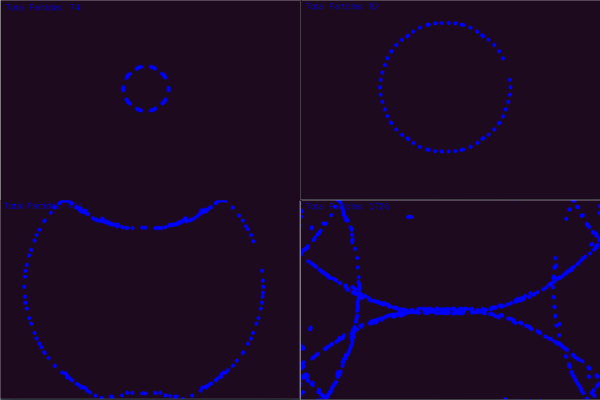
\includegraphics[width=\textwidth]{center.png}
        \caption{Wave expanding from the centre of the window.}
    \end{figure}
    \begin{figure}[H]
        \centering
        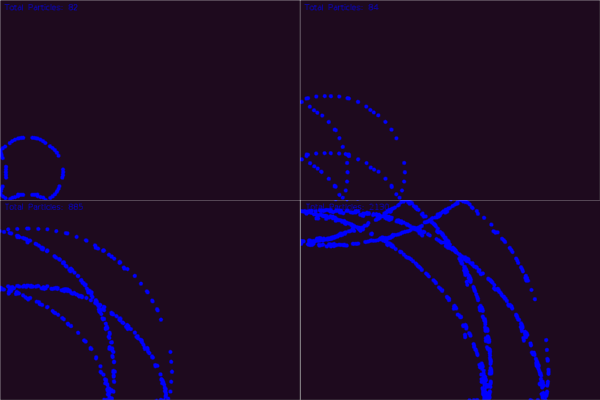
\includegraphics[width=\textwidth]{corner.png}
        \caption{Wave expanding from the corner}
    \end{figure}
    

I didn't implement this on GPU, and used an alternate method to avoid excessive inter-particle distance calculations. 
The implementation simply works by creating new particles as a wave expands in space, specifically 3 particles. However obviously the number of particles increases exponentially as the wave moves through space.
Despite this however I realized that very quickly my dataset of particles would use all the resources of my CPU and slow. 

\section{Next Steps}
As for how I would improve this I would implement this on GPU in either WebGL through shaders or use existing libraries like CUDA.
Seeing as I want to use this to visualize audio travelling through space I'll need to consider how the algorithm will work in 3D and how to translate this resulting data into an audio simulation.

\end{document}
